\chapter{Lensing convergence and neutrino mass in galaxy surveys}
\label{chapter:7}

\section{Introduction}
\label{chapter:7:introduction}

Measurements of the Cosmic Microwave Background (CMB) anisotropies over the past three decades represent a remarkable achievement in cosmology \commentr{cite cobe, wmap, planck papers}. Constant increases in both amount and quality of data not only have allowed more rigorous tests of cosmological models, but also have required the improvement of both the tools and methods we use for the analysis of those data sets. This progress has turned out in a phenomenological model of the universe which fits reasonably well most of the available observations \commentr{cite Planck paper about cosmological parameters}.    

Although the $\Lambda CDM$ model is relatively successful at explaining the current observations, most of the underlying physics in the model remains unknown (e.g., dark energy, dark matter). In particular, the unknown Cold Dark Matter (CDM) constitutes about $30\%$ of the energy content in the universe. Searches for dark matter particles have come out with no conclusive results leaving neutrinos as the only known dark matter candidate. Neutrino experiments have shown that neutrinos are massive particles, but have been unable to provide an absolute scale for their masses \commentr{cite Julien's reviews}. 

Since massive neutrinos change the background evolution of the universe the CMB measurements can be utilised to constraint their masses. When the neutrino mass is small ($\approx 0.1 \, \mathit{eV}$) neutrinos have a modest signature on the CMB angular power spectrum and those constraints can provide only an upper limit for the neutrino mass. Degeneracies with other parameters in the cosmological model (e.g., the equation of state of dark energy $w$ or the Hubble parameter $H_0$) help to further degrade constraints on the neutrino mass from CMB data.  
   
By mapping the distribution of matter in the universe one can also test cosmological models. Galaxy surveys, probing the low red-shift universe, allow to break parameter degeneracies hence improving the constraints on the neutrino masses \commentr{cite paper by W. Hu et al.}. Massive neutrinos would suppress the clustering of galaxies at small scales thus damping the matter power spectrum $P(k)$ on those scales. It is expected that future galaxy surveys will be able to measure this suppression and therefore determine the  absolute mass of the neutrinos.  
  
Future galaxy surveys will probe distance scales comparable to the Hubble horizon (a few tens of $\mathrm{Gpc^3/h^3}$) allowing thus more rigorous analysis. Non-linearities and relativistic effects such as red-shift space distortions and lensing convergence should then be consistently included in galaxy clustering analyses if the constraining power of the survey is not to be wasted. This chapter aims at showing the importance of the inclusion of lensing convergence in galaxy clustering analyses. In particular, we show that if future analyses neglected the lensing convergence, measurements of the neutrino masses would be severely biased thus throwing away valuable information and leading to misleading conclusions about the cosmological model. 

The plan of the chapter is as follows. In the next Section we recall how galaxy number counts are modelled. Our methodology is explained in Section \ref{chapter:7:methodology}. Then in Section \ref{chapter:7:results} we show and discuss our results. Finally, we give our conclusions in Section \ref{chapter:7:conclusions}.

\section{Galaxy number counts angular power spectrum}
\label{chapter:7:modelling}

Although galaxy red-shift surveys measure red-shift $z$ and direction $\mathbf{n}$ of sources in the sky, analyses of galaxy clustering data are commonly done by using the matter power spectrum $P(k,z)$ \commentr{cite Hume's paper 1994} which is not an observable. An alternative approach uses the angular matter power spectrum $C_\ell(z,z')$ which is an observable. It has been shown in \commentr{cite Enea's paper 2013} that for galaxy catalogues with photometric red-shifts, an analysis of the $C_\ell(z,z')$ spectra can perform significantly better than one using $P(k,z)$. This is due to both an optimal use of red-shift information and the not averaging over directions in the $C_\ell(z,z')$ approach. It is therefore more suitable to work with the angular matter power spectrum and we have chosen to do so in this project.  

Galaxy number counts for a survey with limiting magnitude $m_{\mathrm{lim}}$ is given by 
\begin{equation}
\label{Eq:galaxy-number-counts}
n(z,\mathbf{n};\,m_{\mathrm{lim}}) = \bar{n}(z) \left[ 1 + \Delta(z,\mathbf{n};m_{\mathrm{lim}}) \right],
\end{equation}  
where $\bar{n}(z)$ is the mean galaxy density per red-shift and per steradian at red-shift $z$, and 
\begin{eqnarray}
\label{Eq:galaxy-number-counts-perturbation}
\Delta(z,\mathbf{n};m_{\mathrm{lim}}) &=&  b(z) D + \frac{1}{\H}\left[ \dot{\Phi} + \partial_r^2 V \right] + (2 - 5 s) \left[ \int_0^r \frac{d\tilde{r}}{r}(\Phi + \Psi) - \kappa \right] \nonumber \\
&+&  (f_{\mathrm{evo}} - 3)\H V + (5s-2)\Phi + \Psi 
+ \left( \frac{\dot{\H}}{\H^2} + \frac{2 - 5s}{r\H} + 5s - f_{\mathrm{evo}} \right) \nonumber \\
&\times & \left( \Psi + \partial_rV + \int_0^r d\tilde{r}(\dot{\Phi} + \dot{\Psi}) \right) 
\end{eqnarray}
is the perturbation in the number density of sources which emerges due to both red-shift density perturbations and volume distortions  \commentr{cite papers by Ruth, Challinor, and the Asian guys}. In Eq. \eqref{Eq:galaxy-number-counts-perturbation} $b(z)$ takes into account that galaxies are biased tracers of the underlying dark matter distribution, $D$ is the density fluctuation in comoving gauge, $\H \equiv aH$ is the conformal Hubble parameter, $\Phi$ and $\Psi$ are the Bardeen potentials \commentr{Bardeen's paper 1982?}, $V$ is the velocity potential for peculiar velocities in the longitudinal gauge, $v_i=-\partial_i V$, $s$ is the magnification bias , $\kappa$ is the convergence, $r$ is the comoving distance, $f_{\mathrm{evo}}$ is the evolution bias, and a dot denotes derivative w.r.t. conformal time. Both the evolution bias and the magnification bias functions are defined below when giving the survey specifications. 

Similarly to what is done in CMB analysis with temperature fluctuations, it is useful to expand the perturbation in the number density of galaxies in spherical harmonics $Y_{\ell\,m}(\mathbf{n})$. Whereas for the CMB case one expands the temperature fluctuations field $\Delta T(\mathbf{n})$ at a single red-shift ($z\sim 1000$), when analysing galaxy catalogues we have data for a range of red-shifts and therefore the expansion takes into account this red-shift dependence
\begin{equation}
\label{Eq:galaxy-number-counts-perturbation-expansion}
\Delta(z,\mathbf{n}) = \sum_{\ell,m} a_{\ell m}(z) Y_{\ell m}(\mathbf{n}), 
\end{equation}   
where we have omitted the limiting magnitude. Assuming statistical isotropy, it is possible to define the angular matter power spectrum through the expansion \eqref{Eq:galaxy-number-counts-perturbation-expansion} as
\begin{equation}
\label{Eq:definition-angular-matter-power-spectrum}
\langle a_{\ell m}(z) a^*_{\ell m}(z') \rangle \equiv \delta_{\ell \ell'} \delta_{m m'} C_\ell(z,z').
\end{equation} 

In practice, galaxy clustering data is commonly analysed by using tomographically binned samples of galaxies. The catalogue can be divided in different red-shift bins according to normalised window functions $W_{\Delta z_i}(z,z_i)$ of width $\Delta z_i$ and centred in red-shift $z_i$. One can then define correlations between red-shift bins $i$ and $j$ as
\begin{equation}
\label{Eq:binned-angular-matter-power-spectrum}
C_\ell^{ij} \equiv \int dz dz' W_{\Delta z_i}(z,z_i) W_{\Delta z_j}(z,z_j) C_\ell (z,z').
\end{equation} 
In this project we have used synthetic galaxy clustering data for a survey consistent with the Euclid photometric catalogue:
\begin{itemize}
\item the covered sky fraction $f_{\mathrm{sky}}=0.364$; 
\item we divide the catalogue into $N_{\mathrm{bin}}=5$ Gaussian red-shift bins (Gaussian window functions $W_{\Delta z_i}$) containing equal number of galaxies;
\item the galaxy red-shifts are assumed to range from $0.1$ to $2$;
\item the galaxy density $d=30\,\mathrm{arcmin^{-2}}$;
\item the number of galaxies per red-shift and per steradian 
\begin{equation}
\label{Eq:dNdzdOmega}
\dfrac{dN}{dzd\Omega} = 3.5\times 10^8 z^2 \exp \left[-\left( \frac{z}{z_0} \right)^{3/2} \right] \qquad z_0=0.637; 
\end{equation}
\item the number of galaxies per steradian within a given red-shift bin is 
\begin{equation}
\label{Eq:number-galaxies-per-bin}
\N = \frac{1}{N_{\mathrm{bin}}}\int dz \dfrac{dN}{dzd\Omega};
\end{equation}
\item as suggested by previous studies (see, for instance, \commentr{cite SDSS paper ''The three dimensional power spectrum of galaxies from the sloan digital sky survey}) we assume a scale-independent galaxy bias 
\begin{equation}
b(z) = b_0\sqrt{1+z};
\label{Eq:galaxy-bias}
\end{equation}
\item following \commentr{Cite Francesco's paper} the magnification bias for an Euclid-like survey is modelled as 
\begin{equation}
s(z) = \sum_{k=0}^3 s_k z^k,
\label{Eq:magnification-bias}
\end{equation}
with $s_0 = 0.1194,\, s_1 = 0.2122,\, s_2 = -0.0671,\, s_3 = 0.1031$;
\item finally, the evolution bias 
\begin{equation}
f_{\mathrm{evo}}(z) \equiv \dfrac{\partial \ln \left( a^3 \dfrac{dN}{dzd\Omega}  \right)}{\partial \ln a},
\label{Eq:evolution-bias}
\end{equation}    
where $a$ is the scale factor and we assume that the survey observes all the galaxies in the windows.
\end{itemize}   

Having the survey specifications we can compute angular matter power spectrum as in Eq. \eqref{Eq:binned-angular-matter-power-spectrum}. We have utilised the code CLASSgal \commentr{cite Enea's paper} where galaxy number counts have been implemented including relativistic corrections in Eq. \eqref{Eq:galaxy-number-counts-perturbation}. In Figure \ref{Fig:comparison-massive-massless-Cls} we compare galaxy number counts angular power spectrum for a model with massive neutrinos and a model where neutrinos are massless. In the next section we study the importance of including the effect of lensing convergence in galaxy clustering analyses when determining the neutrino mass. 

\begin{figure}[hbtp]
\centering
%\includegraphics[scale=1]{}
\caption{\commentr{Include figure in two columns}Comparison auto and cross-corelations for models with and without neutrino mass}
\label{Fig:comparison-massive-massless-Cls}
\end{figure}
 
\section{Methodology}
\label{chapter:7:methodology}

In order to show the importance of inclusion of lensing convergence in galaxy clustering analyses, we perform a Markov Chain Monte Carlo (MCMC) analysis \commentr{cite paper by Lewis and Sarah B.} both including and neglecting the lensing effect. Studies analysing the bias on cosmological parameters due to neglecting lensing convergence can be found in the literature, but they do Fisher matrix analysis and focus on either the primordial non-Gaussianity (i.e., $\fNL$) \commentr{cite paper by Namikawa} or dark energy parameters (e.g., $w,\, \Omega_\Lambda$) \commentr{cite paper by Alan Heavens}. Although in this project we stress the neutrino mass, we also discuss other parameters in the concordance model.  

The MCMC technique is more suitable than a Fisher matrix method. Current Boltzmann codes such as CLASS \commentr{Julien's paper} or CAMB \commentr{paper by Lewis and Challinor} are accurate to $1\%$ (with nominal precision settings), but it is possible for random numerical errors to exceed this. Future surveys will provide more precise Large Scale Structure (LSS) measurements and therefore these effects might become problematic for approaches that rely on computation of derivatives as a function of parameters (e.g., Fisher matrix). Since our MCMC approach average over $\sim 10^5$ galaxy number counts spectra, it is much less sensitive to those numerical errors than the Fisher matrix approach. 

We assume a fiducial flat $\Lambda CDM$ model consistent with results from the Planck collaboration \commentr{Planck paper cosmological parameters}, including massive neutrinos with a normal mass hierarchy (dominated by the heaviest neutrino mass eigenstate). The cosmological parameters of our fiducial model are the reduced baryon density parameter, $\omega_{\mathrm{b}} = 2.225\times 10^{-2}$, the cold dark matter density parameter, $\omega_{\mathrm{cdm}}=0.1198$, the scalar spectral index, $n_{\mathrm{s}}=0.9645$, the amplitude of curvature fluctuations, $\ln 10^{10} A_{\mathrm{s}}=3.094$, the Hubble constant, $H_0 = 67.27\, \mathrm{km\, s^{-1}\, Mpc^{-1}}$, and the sum of the neutrino masses, $\sum m_\nu = 0.06\, \mathrm{eV}$.  
     
To take into account theoretical error on non-linear scales we use Halofit \commentr{cite reference 52 in Francesco's paper} to rescale all linear transfer functions. The rescaling for the matter power spectrum in models including massive neutrinos has been already implemented in CLASSgal. Transfer functions are rescaled by the square root of 
\begin{equation}
\alpha(k,z) = \frac{\ln [1 + k/k_{\mathrm{NL}(z)}]}{1 + \ln [1 + k/k_{\mathrm{NL}(z)}]}f_{\mathrm{th}},
\label{Eq:rescaling-factor-transfer-functions}
\end{equation}
where $k_{\mathrm{NL}}$ is the non-linear scale determined by the Halofit algorithm, and $f_{\mathrm{th}}$ is the error percentage on non-linear scales which we have chosen to be $f_{\mathrm{th}}=10\%$. The theoretical error power spectra $E_\ell^{ij}$ are then computed by taking the absolute value of the resulting $C_\ell^{ij}$. Because computing $E_\ell^{ij}$ with high accuracy is time-computing demanding, in this project we compute the error power spectra only for the fiducial model, that is, we ignore the parameter dependence on the theoretical error.

Since perturbation on the number density of galaxies is not a continuous field, it is usually assumed that galaxies form a Poisson sample of the density field \commentr{cite paper by Hume et al.} and therefore there is a shot-noise contribution $\N^{-1}$ to the error budget in the angular power spectra.

Finally, the galaxy number counts are modelled as 
\begin{equation}
\label{Eq:GNC-modelled-angular-power-spectra}
C_\ell^{A,\,ij} = C_\ell^{ij} + E_\ell^{ij} + \N^{-1} \delta^{ij},
\end{equation}
where $A=\mathrm{obs},\,\mathrm{th}$ and $i,j = 1,...,N_{\mathrm{bin}}$ are red-shift bin indices. Here $C_\ell^{\mathrm{obs}}$ stands for spectra computed for our fiducial model which includes the effect of lensing convergence, and $C_\ell^{\mathrm{th}}$ stands for models which might or might not include lensing convergence. In the next Section we will see what the impact of switching lensing convergence off in $C_\ell^{\mathrm{th}}$ is when fitting this kind of models to our fiducial $C_\ell^{\mathrm{obs}}$.   
     
Following the cosmic shear implementation in \commentr{cite B. Audren's paper} we have implemented a Gaussian likelihood for an Euclid-like survey. For given observed and theoretical power spectra in Eq. \eqref{Eq:GNC-modelled-angular-power-spectra}, let us define the determinants
\begin{eqnarray}
\label{Eq:determinants-Gaussian-likelihood}
d_\ell^{\mathrm{th}} & = & \det \left( C_\ell^{\mathrm{th},\,ij}\right),\\
d_\ell^{\mathrm{obs}} & = & \det \left( C_\ell^{\mathrm{obs},\,ij}\right). 
\end{eqnarray}
Additionally, one can define a mixed determinant $d_\ell^{\mathrm{mix}}$ formed from $d_\ell^{\mathrm{th}}$: one takes each term in $d_\ell^{\mathrm{th}}$ and replaces one at a time $C_\ell^{\mathrm{th},\,ij}$ by the corresponding $C_\ell^{\mathrm{obs},\,ij}$. If we worked $2$ red-shift bins, the mixed determinant would read
\begin{equation}
\label{Eq:example-mixed-determinant}
d_\ell^{\mathrm{mix}} = C_\ell^{\mathrm{obs},\,11}C_\ell^{\mathrm{th},\,22} + C_\ell^{\mathrm{th},\,11}C_\ell^{\mathrm{obs},\,22} - 2 C_\ell^{\mathrm{th},\,12}C_\ell^{\mathrm{obs},\,12}.
\end{equation}
                        
We know that in an ideal full-sky experiment, the different multipoles in an spherical harmonics expansion of a given function are uncorrelated. Then in this simple case one can write the Gaussian likelihood
\begin{equation}
\label{Eq:GNC-Gaussian-likelihood}
\L = \tilde{\N} \Pi_\ell \left\lbrace \frac{1}{(d_\ell^{\mathrm{th}})^{\frac{2\ell+1}{2}}} \exp \left[ -\frac{(2\ell+1)}{2} \frac{d_\ell^{\mathrm{mix}}}{d_\ell^{\mathrm{th}}}\right] \right\rbrace,                         
\end{equation}
where $\tilde{\N}$ is a normalisation constant. The effective chi square is defined as
\begin{equation}
\label{Eq:GNC-effective-chi2}
\chi^2_\eff \equiv -2 \ln \L = -2 \ln \tilde{\N} + \sum_\ell (2\ell+1)\left( \ln d_\ell^{\mathrm{th}} + \frac{d_\ell^{\mathrm{mix}}}{d_\ell^{\mathrm{th}}} \right), 
\end{equation}
which is minimal for $d_\ell^{\mathrm{mix}}= N_{\mathrm{bin}} d_\ell^{\mathrm{th}} = N_{\mathrm{bin}} d_\ell^{\mathrm{obs}}$. Having into account the partial sky coverage these definitions lead to a $\chi^2$ relative to the fiducial model given by                     
\begin{equation}
\label{Eq:relative-chi2}
\Delta \chi^2 = \sum_{\ell=2}^{\ell_{\mathrm{max}}} (2\ell+1) f_\fsky \left( \ln \frac{d_\ell^{\mathrm{th}} }{d_\ell^{\mathrm{obs}}} + \frac{d_\ell^{\mathrm{mix}}}{d_\ell^{\mathrm{th}}} - N_{\mathrm{bin}} \right),
\end{equation}                           
where to be conservative in the treatment of non-linear effects we use $\ell_{\mathrm{max}}=400$. In order to optimise the computation of the angular power spectra $C_\ell^{\mathrm{A},\,ij}$ we use the Limber approximation and adjust the precision parameters in CLASSgal to have $\Delta \chi^2 \lesssim 0.2$ for $C_\ell^{\mathrm{th}}$ including lensing evaluated at the fiducial model. These adjustments are necessary to make feasible our MCMC approach and mean that our computations are accurate up to $\Delta \chi^2 \lesssim 0.2$.                              
                     
With the approach explained above we have performed three analyses, namely:
\begin{enumerate}
\item $C_\ell^{\mathrm{th}}$ including lensing convergence.
\item $C_\ell^{\mathrm{th}}$ neglecting lensing convergence.
\item $C_\ell^{\mathrm{th}}$ neglecting lensing convergence, but including only auto-correlations.
\end{enumerate}
                                                  
\section{Results}
\label{chapter:7:results}

We have performed the three analyses previously mentioned in two ways. First, we assume no knowledge about cosmological parameters and use flat priors. Second, we have added CMB information by using Gaussian priors with widths given by the Planck results for their analysis which have a varying neutrino mass. 

\subsection{Flat prior}

\begin{table}[!t]
\centering
\begin{tabular}{@{}cccccc}
\hline
\multicolumn{6}{c}{i) Consistently including lensing: $\Delta \chi^2 = 0.075$} \\
\hline
Parameter & Mean & best fit & $\sigma$ &\hspace{-0.52cm} shift: mean & best-fit \\
\hline
$\omega_b$ & $0.02979$ & $0.02285 $ &$0.00624 $ &  \quad$1.2\sigma$ & $ 0.1\sigma$ \\
$\omega_{cdm}$ & $0.1455 $ & $0.1219 $ & \quad$0.0200 $ &  \quad$1.3\sigma$ & $0.1\sigma$ \\
$n_s$      & $0.9476 $ & $0.9642 $ & $0.0387 $ &  \quad$0.4\sigma$ & $ <0.1\sigma$ \\
$\ln10^{10}A_s$ & $3.047 $ & $3.097$ & $0.065 $ &  \quad$0.7\sigma$ & $ <0.1\sigma$ \\
$H_0\left[\frac{\text{km}}{\text{s}\cdot\text{Mpc}}\right]$      & $73.84$ & $67.84$ & $5.48$ &  \quad$1.2\sigma$ & $ 0.1\sigma$ \\
$m_{\nu}$\,[eV]  & $0.29$ & $0.09$ & $0.19$ & \quad $ 1.2\sigma$ & $ 0.2\sigma$ \\
$b_0$ & $1.018$ & $1.000$ & $0.031$ & $0.6\sigma$ & $<0.1\sigma$ \\
\end{tabular}
\begin{tabular}{@{}cccccc}
\hline
\multicolumn{6}{c}{ii) Neglecting lensing: $\Delta \chi^2 = 2063.922$} \\
\hline
Parameter & Mean & best fit & $\sigma$ & \hspace{-0.52cm} shift: mean & best-fit \\
\hline
$\omega_b$ & $0.02494$ & $0.02120 $ & $0.00556 $ &  \quad$0.5\sigma$ & $0.1\sigma$ \\
$\omega_{cdm}$ & $0.1532$ & $0.1435$ & $0.0208$ &  \quad$1.6\sigma$ & $1.1\sigma$ \\
$n_s$      & $0.8702$ & $0.8837$ & $0.0446$ &  \quad$2.1\sigma$ & $1.8\sigma$ \\
$\ln10^{10}A_s$ & $ 2.867 $ & $2.965 $ & $ 0.394 $ &  \quad$0.6\sigma$ & $0.3\sigma$ \\
$H_0\left[\frac{\text{km}}{\text{s}\cdot\text{Mpc}}\right]$      & $68.73$ & $66.76$ & $5.14$ &  \quad$0.3\sigma$ & $0.1\sigma$ \\
$m_{\nu}$\,[eV]  & $0.43$ & $0.41$ & $0.16$ &  \quad$2.3\sigma$ & $2.2\sigma$ \\
$b_0$ & $1.293$ & $1.200$ & $0.271$ & $1.1\sigma$ & $0.7\sigma$\\
\end{tabular}
\begin{tabular}{@{}cccccc}
\hline
\multicolumn{6}{c}{\parbox[t]{4.4cm}{iii) Neglecting lensing: \\(only auto-correlations)} $\Delta \chi^2 = 180.254$} \\
\hline
Parameter & Mean & best fit & $\sigma$ & \hspace{-0.52cm} shift: mean & best-fit\\
\hline
$\omega_b$ & $0.01982 $ & $0.01737 $ & $0.00520 $ &  \quad$0.5\sigma$ & $0.9\sigma$ \\
$\omega_{cdm}$ & $0.1658 $ & $0.1552 $ & $0.0242 $ &  \quad$1.9\sigma$ & $1.5\sigma$ \\
$n_s$      & $0.7539 $ & $0.7675 $ & $0.0513 $ &  \quad$4.1\sigma$ & $3.8\sigma$ \\
$\ln10^{10}A_s$ & $2.449 $ & $2.719 $ & $0.465 $ &  \quad$1.4 \sigma$ & $0.8\sigma$ \\
$H_0\left[\frac{\text{km}}{\text{s}\cdot\text{Mpc}}\right]$      & $61.64 $ & $59.11$ & $5.43$ &  \quad$1 \sigma$ & $1.5\sigma$ \\
$m_{\nu}$\,[eV]  & $0.41$ & $0.41$ & $0.14$ &  \quad$2.6\sigma$ & $2.5\sigma$ \\
$b_0$ & $1.888$ & $1.603$ & $0.428$ & $2.1\sigma$ & $1.4\sigma$ \\
\end{tabular}

\caption{MCMC results (flat prior). We show the mean and best fit values, the standard deviation and the amplitude of the shift of the mean and best-fit w.r.t the fiducial value in units of the standard deviation, $\sigma$, of the corresponding analysis. The large value of $\Delta \chi^2$ for case ii) shows that cross-correlations cannot be fitted if lensing is neglected.
}
\label{Table:mcmc-flat-prior}
\end{table}

\begin{figure}[bthp]
\centering
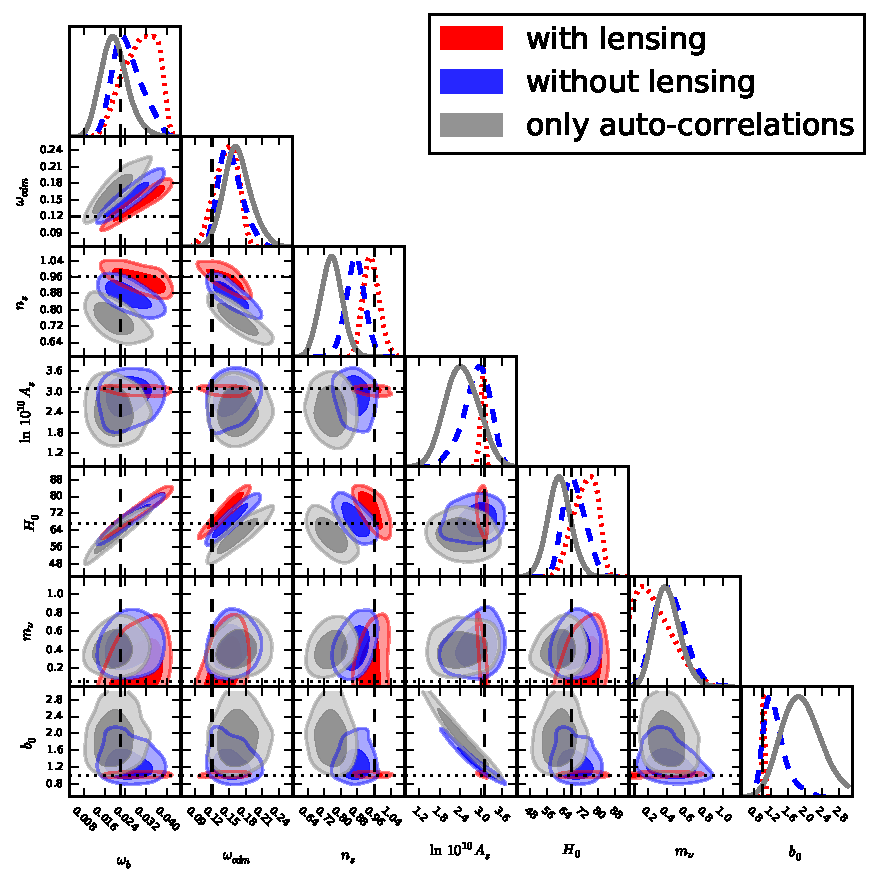
\includegraphics[scale=1]{figures/chapter-7/triangle_figure_MCDM_bias.pdf} 
\caption{Two- and 1-D posteriors for the cosmological parameters inferred from the full analysis including lensing (red dotted), an analysis neglecting lensing (blue dashed) and considering only auto-correlations (gray solid).
{The $68\%$ and $95\%$ confidence intervals are shown.}
Intersections between vertical and horizontal lines denote the fiducial cosmology.
}
\label{Fig:mcmc-flat-prior}
\end{figure}

\commentr{triangle plot and table. Discuss degeneracies, bias, current limits in neutrino mass, and show spectra for best fits}

\subsection{Gaussian prior}

\commentr{triangle plot and table. Conclusions change w.r.t to flat priors ?}

\begin{table}[!t]
\centering
\begin{tabular}{@{}cccccc}
\hline
\multicolumn{6}{c}{i) Consistently including lensing: $\Delta \chi^2 = 768.443$} \\
\hline
Parameter & Mean & best fit & $\sigma$ &\hspace{-0.52cm} shift: mean & best-fit \\
\hline
$\omega_b$ & $0.02225$ & $0.02225 $ &$0.00016 $ &  \quad$<0.1\sigma$ & $ <0.1\sigma$ \\
$\omega_{cdm}$ & $0.1202 $ & $0.1203 $ & \quad$0.0013 $ &  \quad$0.3\sigma$ & $0.4\sigma$ \\
$n_s$      & $0.9652 $ & $0.9636 $ & $0.0044 $ &  \quad$0.2\sigma$ & $ 0.2\sigma$ \\
$\ln10^{10}A_s$ & $3.090 $ & $3.092$ & $0.045 $ &  \quad$0.1\sigma$ & $ <0.1\sigma$ \\
$H_0\left[\frac{\text{km}}{\text{s}\cdot\text{Mpc}}\right]$      & $67.09$ & $67.16$ & $0.82$ &  \quad$0.2\sigma$ & $ 0.1\sigma$ \\
$m_{\nu}$\,[eV]  & $0.09$ & $0.08$ & $0.06$ & \quad $ 0.5\sigma$ & $ 0.3\sigma$ \\
$b_0$ & $1.006$ & $1.004$ & $0.026$ & $0.2\sigma$ & $0.2\sigma$ \\
\end{tabular}
\begin{tabular}{@{}cccccc}
\hline
\multicolumn{6}{c}{ii) Neglecting lensing: $\Delta \chi^2 = 2847.399$} \\
\hline
Parameter & Mean & best fit & $\sigma$ & \hspace{-0.52cm} shift: mean & best-fit \\
\hline
$\omega_b$ & $0.02221$ & $0.02221 $ & $0.00017 $ &  \quad$0.2\sigma$ & $0.2\sigma$ \\
$\omega_{cdm}$ & $0.1212$ & $0.1207$ & $0.0015$ &  \quad$1\sigma$ & $0.6\sigma$ \\
$n_s$      & $0.9638$ & $0.9637$ & $0.0049$ &  \quad$0.1\sigma$ & $0.2\sigma$ \\
$\ln10^{10}A_s$ & $ 2.368 $ & $2.446 $ & $ 0.428 $ &  \quad$1.7\sigma$ & $1.5\sigma$ \\
$H_0\left[\frac{\text{km}}{\text{s}\cdot\text{Mpc}}\right]$      & $65.83$ & $65.96$ & $0.92$ &  \quad$1.6\sigma$ & $1.4\sigma$ \\
$m_{\nu}$\,[eV]  & $0.35$ & $0.33$ & $0.06$ &  \quad$4.8\sigma$ & $4.5\sigma$ \\
$b_0$ & $1.574$ & $1.479$ & $0.339$ & $1.7\sigma$ & $1.4\sigma$\\
\end{tabular}
\begin{tabular}{@{}cccccc}
\hline
\multicolumn{6}{c}{\parbox[t]{4.4cm}{iii) Neglecting lensing: \\ \hspace*{0.9cm} (only auto-correlations)} $\Delta \chi^2 = 998.208$} \\
\hline
Parameter & Mean & best fit & $\sigma$ & \hspace{-0.52cm} shift: mean & best-fit\\
\hline
$\omega_b$ & $0.02219 $ & $0.02219 $ & $0.00017 $ &  \quad$0.3\sigma$ & $0.4\sigma$ \\
$\omega_{cdm}$ & $0.1222 $ & $0.1221 $ & $0.0014 $ &  \quad$1.7\sigma$ & $1.6\sigma$ \\
$n_s$      & $0.9640 $ & $0.9646 $ & $0.0050 $ &  \quad$0.1\sigma$ & $<0.1\sigma$ \\
$\ln10^{10}A_s$ & $1.672 $ & $1.488 $ & $0.427 $ &  \quad$3.3 \sigma$ & $3.8\sigma$ \\
$H_0\left[\frac{\text{km}}{\text{s}\cdot\text{Mpc}}\right]$      & $63.90 $ & $63.89$ & $0.98$ &  \quad$3.4 \sigma$ & $3.4\sigma$ \\
$m_{\nu}$\,[eV]  & $0.49$ & $0.49$ & $0.06$ &  \quad$7.1\sigma$ & $7\sigma$ \\
$b_0$ & $2.295$ & $2.461$ & $0.454$ & $2.9\sigma$ & $3.2\sigma$ \\
\end{tabular}

\caption{MCMC results (Gaussian prior). We show the mean and best fit values, the standard deviation and the amplitude of the shift of the mean and best-fit w.r.t the fiducial value in units of the standard deviation, $\sigma$, of the corresponding analysis. The large value of $\Delta \chi^2$ for case ii) shows that cross-correlations cannot be fitted if lensing is neglected.
}
\label{Table:mcmc-gaussian-prior}
\end{table}


\begin{figure}[bthp]
\centering
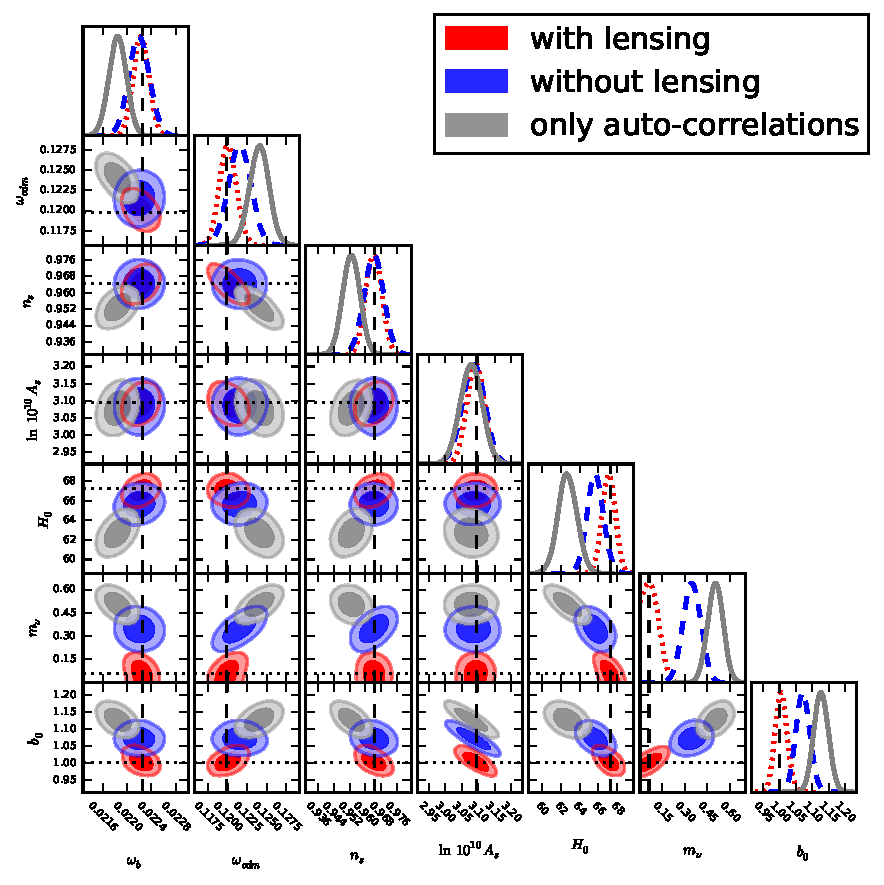
\includegraphics[scale=1]{figures/chapter-7/triangle_figure_MCDM_bias_cmb_prior.pdf}
\caption{Two- and 1-D posteriors for the cosmological parameters inferred from the full analysis including lensing (red dotted), an analysis neglecting lensing (blue dashed) and considering only auto-correlations (gray solid).
{The $68\%$ and $95\%$ confidence intervals are shown.}
Intersections between vertical and horizontal lines denote the fiducial cosmology.
}
\label{fig:mcmc-cmb-prior}
\end{figure}
\section{Conclusions}
\label{chapter:7:conclusions}

\commentr{lensing convergence must be included in galaxy clustering analysis. LSS breaks degeneracies.}

%The study of the large scale structure of the universe allows us to test the different cosmological models. The sky coverage and the deepness in redshift of  galaxy surveys have improved significantly in the past decades. This, in addition to the high precision CMB experiments, will able us to break the degeneracies in cosmological models that have plagued cosmology for quiet a while already. In particular, a better mapping of the matter distribution in the universe will help to put tighter constraints on the masses of neutrinos. Indeed, the clustering properties of the mass in the universe depend on the neutrino masses and possibly on their hierarchy. 

%Due to the experiments carried out in particle accelerators we know that neutrinos are massive. Nevertheless, we do not have a precise estimation for their masses which, in turn, unable us to estimate their total contribution to the energetic composition of the universe. Therefore, by measuring precisely the neutrino masses we can discriminate between different cosmological models since these predict distinct clustering properties. 

%In this chapter we do forecasts on the neutrino masses by using an Euclid-like survey. We use formalism of the angular power spectrum of the matter distribution and include the relevant relativistic effects, namely, lensing and redshift space distortions. The advantage of this formalism over the usual power spectrum $P(k;\, z=z_0)$ is that \dots \texttt{I must have a review of the literature and understand much better the two formalisms. A first advantage is related to the fact that the $C_{\ell}$ formalism deals with quantities which are directly observable without any model assumption. \\
%In the Euclid teleconference of Monday 14.12.2014 a Italian guy mentioned a third formalism. \\
%In particular, it would be important to understand why we include only the relativistic effects above. \\
%In addition, I must clarify the differences between spectroscopy and tomographic surveys. \\
%In connection with this last point, I should make clear what the power of Euclid will be.}

%In summary, in this chapter we aim to answer the following questions. First, will Euclid be able to measure the neutrino masses ?. Second, what error do we expect for such a survey ?. Third, will we be able to distinguish between different hierarchies with a Euclid-like survey ? 
